\section{Theoretical Basics}
\label{sec:3_theoretical_basics}

In order to fully understand our work,
it is important to ensure a few basics in the area of \Gls{nlp}.
In this chapter we will explain how the most important techniques used in our thesis work.

\subsection{Text Preprocessing}
\label{subsec:3_text_preprocessing}

When working with text data, many algorithms and methods will need to distinguish words from another.
In most cases this is done by creating a dictionary of all known words and by \textit{vectorizing} the text data
according to the dictionary.

While this works well in theory, we deal with a tremendous amount of data in real world applications.
This results in huge directories with many vector dimensions and does not only take up more disk space
but also text processing (computation and comparison) takes more time to process.

What does that mean?
Consider the following words:

\begin{itemize}
    \item switzerland
    \item Switzerland
    \item SWITZERLAND
\end{itemize}

Anyone of us will be able to extract the same meaning out of these three words: The country \textit{Switzerland}.
However, for machines the terms are different to another because they are written differently.
That is why in most cases it makes sense to lowercase all text before processing them.
That way we can ensure that the above words also share the same meaning
for a machine and thus reduce the dictionary size.

\paragraph{Exceptions}
There are a few use cases where lowercasing a text is not desired.
For example when trying to detect the writer's sentiment.
Someone who would write a few or all words of a sentence in uppercase might be angrier than someone who does not.

\paragraph{Reducing the dictionary size}
Lowercasing text can just be the beginning though.
Depending on the size of a document, it might make sense to not use all text data inside a document.
A good example for this would be books.
Vectorizing books would take too much computational power and time to process.
In such cases, the dictionary size needs to be reduced.
This could be accomplished by processing a summary of the book instead of the book itself
or by extracting the most relevant words from the whole book.
Later could be done with Keyphrase Extraction or with \Gls{ner}.

\paragraph{Normalizing text}
If we are not dealing with books but with articles or papers,
there are also other alternatives to Keyphrase Extraction and \Gls{ner}.
Using \textbf{Text Stemming} (\subsubsecref{subsubsec:3_text_stemming})
or \textbf{Text Lemmatization} (\subsubsecref{subsubsec:3_text_lemmatization}),
we can simplify terms and group them together to reduce
the dictionary size.

\subsubsection{Keyphrase Extraction}
\label{subsubsec:3_keyphrase_extraction}

When describing any kind of data, a popular thing to do is tagging.
One of the most well-known tagging procedures are the usage hash tags and user names in social media.
Let us check following Tweet from the \textit{European Space Agency}\cite{ESATweet}:

\begin{quotation}
    This walking and hopping \textbf{\#robot} is currently being tested in ESA’s Mars Yard
    at our \textbf{\detokenize{@ESA_Tech}} centre in the Netherlands.
    SpaceBok is a quadruped robot designed by a Swiss student team from \textbf{\detokenize{@ETH}}
    and \textbf{\detokenize{@ZHAW}}.
\end{quotation}

If we only read the hash tags and user names \textit{\#robot}, \textit{\detokenize{@ESA_Tech}},
\textit{\detokenize{@ETH}} and \textit{\detokenize{@ZHAW}},
we do not retrieve all information but we can already think of what the Tweet is about.
These words would be our \textit{Keyphrases}.

Now, in above example the Keyphrases were defined manually by a user.
But in our data set (and most data sources), there are no Keyphrases.
Luckily there are different approaches on how to retrieve Keyphrases from text data.

We are using SGRank\cite{SGRank} in our thesis as it is currently one of the most used
Keyphrase Extraction algorithms.
Our goal is to check if working with Keyphrases alone is more, less or equal accurate
than with the whole text.

Since the dictionary size would be smaller, the data processing time could be improved.

\subsubsection{Named Entity Recognition}
\label{subsubsec:3_named_entity_recognition}

Similar to \textit{Keyphrase Extraction}, \Gls{ner} extracts relevant terms out from a given text.
However, it does not only extract terms but also states what kind of term it is.
Consider following sentence:

\begin{quotation}
    CERN in Geneva pays tribute to Murray Gell-Mann, who won the Nobel Prize in Physics in 1969.
\end{quotation}

When using spaCy's \gls{ner} model, which is based on a transition-based \gls{cnn}\cite{LampleBSKD16},
we retrieve following entities:

\begin{itemize}
    \item CERN (Organisation)
    \item Geneva (Location)
    \item Murray Gell-Mann (Person)
    \item the Nobel Prize in Physics (Work of art)
    \item 1969 (Date)
\end{itemize}

For comparison, the same sentence would extract following \textit{Keyphrases}:

\begin{itemize}
    \item Nobel Prize
    \item Murray Gell
    \item tribute
    \item Mann
    \item Geneva
    \item Physics
    \item CERN
\end{itemize}

Comparing the numbers of the extracted terms solely, Keyphrase Extraction seems to have delivered a better job.
However, when evaluating the results, we can see that \Gls{ner} \textit{understood} the terms and their
relations better.

Not only was it able to correctly keep the subject's name, \textit{Murray Gell-Mann}, but also the type of Nobel prize.

% TODO: Talk about time.

\subsubsection{Text Stemming}
\label{subsubsec:3_text_stemming}

Text Stemming is a form of Text Normalization which aims to simplify words
by reducing the inflectional forms of each word into their word stems.
For example, the words \textit{connected}, \textit{connecting}, \textit{connection} share a similar meaning and could
therefor be simplified to the base term \textbf{connect}.

The first paper describing a stemming algorithm was written by Julie Beth Lovins\cite{LovinsStemmer}
as early as in 1968.
In her algorithm she used an ordered list of 294 suffixes to strip them out and then applies one of
29 associated application rules followed by a set of 35 rules to check if the remaining stem has to be
modified furtherly.

Lovins' stemming algorithm was very successful but got mostly replaced by
M.F. Porters stemming algorithm\cite{PorterStemmerAlgorithm} published in 1980.
In his paper, M.F. Porter was able to process his suffix stripping algorithm in 6,370 out of 10,000 words and thereby
reducing the vocabulary size by \textbf{one third}.
The algorithm simply follows 5 steps with replacement and/or removal rules and is therefor very easy and efficient.

M.F. Porter improved his stemming algorithm even further
by publishing the Porter2 stemming algorithm\cite{SnowballStemmerAlgorithm} in 2002
which is widely known as the \textit{Snowball stemming algorithm}.

There are even more stemming algoriths, very well known are the Lancester stemming algorithm\cite{LancesterStemmer}
and the WordNet stemming algorithm\cite{WordNetStemmer}.
Since M.F. Porter's snowball stemming algorithm is the most widely used one, we decided to go with his algorithm.

\subsubsection{Text Lemmatization}
\label{subsubsec:3_text_lemmatization}

Similar to \textit{Text Stemming}, Text Lemmatization has the same goal to group together the inflected forms of a word
but follows a different approach to do so.
Instead of processing terms with fixed steps and defined rules,
Text Lemmatization normally includes a dictionary lookup for the words
and also takes in consideration to which part of a sentence a term belongs to.
This results in more accurate root terms but also asks for more computational power than Text Stemming.
See following table for a comparison:

\begin{table}[h]
    \centering
    \begin{tabular}{|l|l|r|r|}
    \hline
    \textbf{\#} & \textbf{Original word} & \textbf{Stemmed} & \textbf{Lemmatized} \\ \hline
    1 & written & written & write \\ \hline
    2 & greatest & greatest & great \\ \hline
    3 & best & best & best \\ \hline
    4 & fastest & fastest & fastest \\ \hline
    5 & highest & highest & high \\ \hline
    6 & compute & comput & compute \\ \hline
    7 & computer & comput & computer \\ \hline
    8 & computed & comput & compute \\ \hline
    9 & computing & comput & compute \\ \hline
    10 & studies & studi & study \\ \hline
    11 & studying & studi & study \\ \hline
    12 & university & univers & university \\ \hline
    13 & universities & univers & university \\ \hline
    14 & universe & univers & universe \\ \hline
    15 & universal & univers & universal \\ \hline
    \end{tabular}
    \caption{Comparison of Text Stemming and Text Lemmatization.}
    \label{tab:comparison_stemming_lemmatization}
\end{table}

% TODO: Talk about time.

\subsection{Vector Space Model}
\label{subsec:3_vector_space_model}

Comparing text documents with each other is not a straightforward task to do.
This is the reason why the \gls{vsm} was developed.

When working with a \gls{vsm}, text documents get vectorized.
This is succeeded by assigning each unique term over all documents to one dimension.

When we now want to compare two documents with each other,
we simply compare their vectors with each other.

But how do we vectorize each term of each document to a numerical value?
Let us have a look at the two most used text vectorizers.

\subsubsection{Term Frequency}
\label{subsubsec:3_term_frequency}

The easiest vectorizer is the Term Frequency Vectorizer.
After creating the dictionary of all used terms, it simply sums up the occurrences for each term.
Consider following three sentences:

\begin{itemize}
    \item Rosetta space probe scopes out landing zone.
    \item Landing site search for Rosetta narrows.
    \item Major Bank Shake-up At Bank of England.
\end{itemize}

After removing \Glspl{stop_word}, we receive 13 unique terms over all documents.
As the Term Frequency Vectorizer simply sums the occurences of each term up,
the \Gls{vsm} looks as in \tabref{tab:tf_vsm}.

\begin{table}[h]
    \centering
    \scalebox{0.85}{
        \begin{tabular}{rrrrrrrrrrrrr}
        \hline
           bank &   england &   landing &   major &   narrows &   probe &   rosetta &   scopes &   search &   shake &   site &   space &   zone \\
        \hline
          0.000 &     0.000 &     1.000 &   0.000 &     0.000 &   1.000 &     1.000 &    1.000 &    0.000 &   0.000 &  0.000 &   1.000 &  1.000 \\
          0.000 &     0.000 &     1.000 &   0.000 &     1.000 &   0.000 &     1.000 &    0.000 &    1.000 &   0.000 &  1.000 &   0.000 &  0.000 \\
          2.000 &     1.000 &     0.000 &   1.000 &     0.000 &   0.000 &     0.000 &    0.000 &    0.000 &   1.000 &  0.000 &   0.000 &  0.000 \\
        \hline
        \end{tabular}
    }
    \caption{Term Frequency \Gls{vsm}.}
    \label{tab:tf_vsm}
\end{table}

We can quickly see that the first two sentences share a few terms
while they do not share any terms with the third sentence.
At the same time we see that the term bank has been used twice in the third sentence.

\subsubsection{tf-idf}
\label{subsubsec:3_tf_idf}

Relying on the Term Frequency alone is a good start but can surely be improved.
Consider following scenario:
We have a document \textit{d1} with 100 terms, 10 of them (10 \%) belong to one specific term \textit{t1}.
In a second document \textit{d2} with 1,000 terms, 10 of them (1 \%) belong to the same term \textit{t1}.
When using Term Frequency as a Vectorizer, both documents will receive for the term \textit{t1} a value of 10.
However, in the first document \textit{d1} the term should have received a higher value
than in document \textit{d2} as it covered a bigger percentage of the document.

This is what tf-idf tries to fix.
Tf-idf was first introduced in 1975 by G. Salton, A. Wong and C. S. Yang \cite{salton1975}
and defines the equation as displayed in \equref{equ:tfidf}.

\begin{equation}
    w_{x,y} = tf_{x,y} \cdot log(\frac{N}{df_x})
    \label{equ:tfidf}
\end{equation}

where $tf_{x,y}$ is the Term Frequency of $x$ in $y$, $N$ the total number of documents
and $df_x$ the documents containing $x$.

However, it is important to note that nowadays there are different tf-idf implementations.
As we are using the scikit-learn\cite{scikit-learn} library,
the tf-idf implementation\cite{scikit_tfidf} of the library is slightly different,
see \equref{equ:scikit_tfidf}.

\begin{equation}
    w_{x,y} = tf_{x,y} \cdot (log(\frac{1+N}{1+df_x}) + 1)
    \label{equ:scikit_tfidf}
\end{equation}

where $tf_{x,y}$ is defined as the equal number of times that term ${_x}$ occurs in document ${_y}$.

If we now calculate the tf-idf value for the term \textit{bank} inside the third document (sentence),
we receive following value: $3.386$.
What scikit-learn now does is to normalize this value using the Euclidean norm:

\begin{equation}
    v_{norm} = \frac{v}{||v||_2} = \frac{v}{\sqrt{v_1{^2}+v_2{^2}+...+v_n{^2}}}
    \label{equ:euclidean}
\end{equation}

This results in following values in our \Gls{vsm}:

\begin{table}[h]
    \centering
    \scalebox{0.85}{
        \begin{tabular}{rrrrrrrrrrrrr}
        \hline
           bank &   england &   landing &   major &   narrows &   probe &   rosetta &   scopes &   search &   shake &   site &   space &   zone \\
        \hline
          0.000 &     0.000 &     0.335 &   0.000 &     0.000 &   0.440 &     0.335 &    0.440 &    0.000 &   0.000 &  0.000 &   0.440 &  0.440 \\
          0.000 &     0.000 &     0.373 &   0.000 &     0.490 &   0.000 &     0.373 &    0.000 &    0.490 &   0.000 &  0.490 &   0.000 &  0.000 \\
          0.756 &     0.378 &     0.000 &   0.378 &     0.000 &   0.000 &     0.000 &    0.000 &    0.000 &   0.378 &  0.000 &   0.000 &  0.000 \\
        \hline
        \end{tabular}
    }
    \caption{tf-idf \Gls{vsm}.}
    \label{tab:tfidf_vsm}
\end{table}

As we can see in \tabref{tab:tfidf_vsm}, the term \textbf{bank} has in document \textit{d3}
a rather high value.
This is because the term is not present in documents \textit{d1} or \textit{d2} but appears
twice in document \textit{d3}.
We can also observe that the term \textbf{rosetta} has slightly different values for the
documents \textit{d1} and \textit{d2}.
The reason for this is that document \textit{d2} has one term less than document \textit{d1},
therefor the significance of one term is weighted heavier in document \textit{d2}.

\subsection{Clustering}
\label{subsec:3_clustering}

Clustering finds similarities in different news articles based on their content and groups them together,
while unrelated news are regarded as noise.
The challenge now arises to find an appropriate clustering method,
which is able to work with data of varying densities and of high dimensionality.

% TODO why hdbscan

\subsubsection{\textit{k}-means clustering}
\label{subsubsec:3_kmeans_clustering}

\textit{k}-means clustering is an iterative clustering method which assigns all data points in a given data set
into k clusters, where k is a predefined number of clusters in the data set.

\paragraph{How does \textit{k}-means clustering work}
At the very beginning, \textit{k}-means creates k centroids at random locations.
It then repeats following instructions until reaching convergence:

\begin{itemize}
    \item For each data point: Find the nearest centroid
    \item Assign the data point to the nearest centroid (cluster)
    \item For each cluster: Compute a new cluster centroid with all assigned data points
\end{itemize}

\paragraph{Advantages}
\begin{itemize}
    \item Very simple and easy to understand algorithm
\end{itemize}

\paragraph{Disadvantages}
\begin{itemize}
    \item Initial (random) centroids have a strong impact on the results
    \item The number of clusters (k) has to be known beforehand
    \item Unable to handle noise (all data points will be assigned to a cluster)
\end{itemize}

\subsubsection{DBSCAN}
\label{subsubsec:3_dbscan}

DBSCAN stands for \textit{Density-Based Spatial Clustering of Applications with Noise}
and is a density based clustering algorithm.

A big advantage of DBSCAN is that it is able to sort data into clusters
of different shapes.

\paragraph{How DBSCAN works}
DBSCAN requires two parameters in order to work:

\begin{enumerate}
    \item epsilon - The maximum distance between two data points for them to be considered as in the same cluster.
    \item minPoints - The number of data points a neighbourhood has to contain in order to be considered as a cluster.
\end{enumerate}

Having these two parameters defined, DBSCAN will iterate through the data points
and try to assign them to clusters if the provided parameters match.
If a data point can not be assigned to a cluster, it will be marked as noise point.

Data points that belong to a cluster but do not dense themselves are known as \textbf{border points}.
Some border points could theoretically belong to two or more clusters
if the distance from the point to the clusters do not differ.

\paragraph{Advantages}
\begin{itemize}
    \item Does not need to know the number of clusters beforehand.
    \item Is able to find shaped clusters.
    \item Is able to handle noise points.
\end{itemize}

\paragraph{Disadvantages}
\begin{itemize}
    \item DBSCAN is not entirely deterministic.
    \item Defining the right epsilon value can be difficult.
    \item Unable to cluster data sets with large differences in densities.
\end{itemize}

\subsubsection{HDBSCAN}
\label{subsubsec:3_hdbscan}

HDBSCAN is a hierarchical density-based clustering algorithm \cite{McInnes2017},
based on DBSCAN and improves its sensitivity for clusters of varying densities.
Therefore defining an epsilon parameter, which acts as a threshold for finding clusters, is no longer necessary.
This makes the algorithm more stable and flexible for different applications.

\paragraph{How HDBSCAN works}
Since HDBSCAN is the focus for this thesis, we want to give a more detailed explanation of its inner workings,
than for \textit{k}-means or DBSCAN.

HDBSCAN only requires one parameter to be set beforehand:

\begin{enumerate}
    \item minPoints - The number of data points a neighbourhood has to contain in order to be considered as a cluster.
\end{enumerate}

The algorithm consist of five steps, which are as follows: 

\subparagraph{1. Transforming the space}
At its core HDBSCAN is a single linkage clustering, which are typically rather sensitive to noise.
A single noise point between clusters could act a bridge, which would result in both clusters to be seen as one.
To reduce this issue, the first step is to increase the distances of lower density points.
This is achieved by to comparing the core distances between two points with the original distance
to get the the mutual reachability distance.
The core distance $core_k(x)$ is defined as the radius of a circle around point $x$,
so that $k$ neighbours are contained within this circle.
TODO describe example in \figref{fig:hdbscan_1}.

\begin{figure}[h]
    \centering
    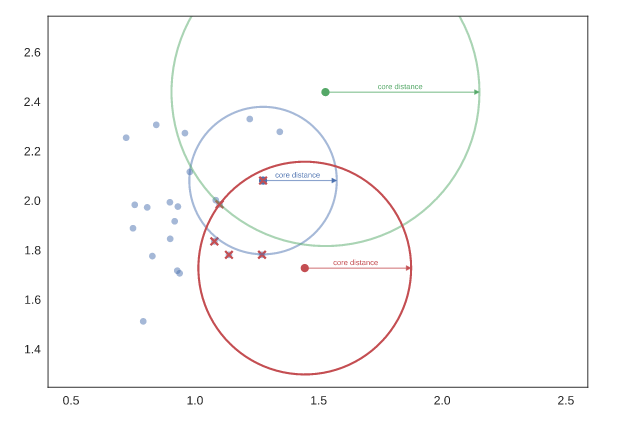
\includegraphics[width=0.5\textwidth]{hdbscan_1}
    \caption{The core distances for three points shown as circles. Source\cite{how_hdbscan_works}}
    \label{fig:hdbscan_1}
\end{figure}

Once the core distances are known, the mutual reachability distance between two points is defined as follows:

\begin{equation*}
    d_{mreach}(a, b) = max\{core_k(a), core_k(b), d(a, b)\}
\end{equation*}

where $d(a, b)$ is the original distance between $a$ and $b$.
Therefore if two points are close together, but the density around one point is rather low,
the core distance will be greater than the original distance and thus the two points appear to be less close together
when considering the mutual reachability distance.

\subparagraph{2. Build the minimum spanning tree}
Based on the mutual reachability distances, the next step is to find points close to each other.
This is done by creating a minimum spanning tree,
where edges are weighted according to the mutual reachability distance and a point is represented by a vertex.
The minimum spanning tree is created one edge at a time,
always choosing the lowest distance to a vertex not yet in the tree.
This is done until each vertex is connected, which results in the minimal set of edges,
such that dropping any edge will cause the disconnect of one or more vertices from the tree.

\subparagraph{3. Build the cluster hierarchy}
Once the minimum spanning tree is complete, it is converted into a hierarchy of connected clusters,
by sorting edges of the tree by distance and iterate through, creating a new merged cluster for each edge.
The dendogram in \figref{fig:hdbscan_2} shows a possible cluster hierarchy. %TODO rewrite this paragraph.

\begin{figure}[h]
    \centering
    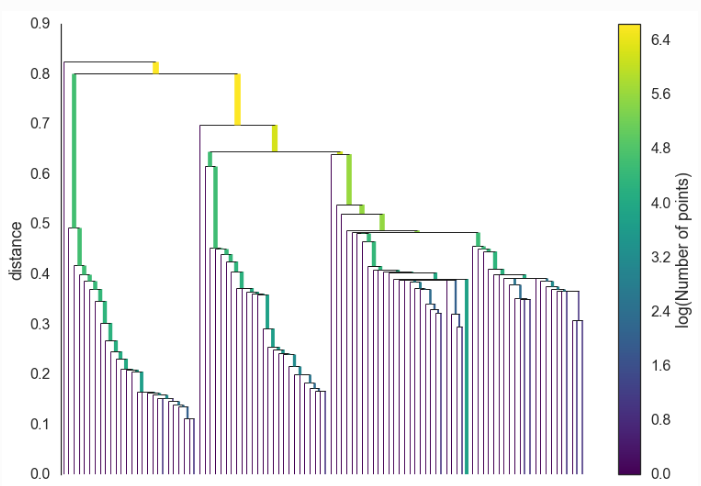
\includegraphics[width=0.5\textwidth]{hdbscan_2}
    \caption{The cluster hierarchy shown as a dendogram. Source\cite{how_hdbscan_works}}
    \label{fig:hdbscan_2}
\end{figure}

At this stage we have to flatten the hierarchy to get the final clusters,
which provide the best representation of the current data set.
DBSCAN simply cuts through the hierarchy using a fixed parameter, usually called epsilon, to get the final clusters.
This approach does not work well with clusters of varying densities and the epsilon parameter itself is unintuitive,
requiring further exploration to find optimal values.
This is were HDBSCAN improves upon DBSCAN, by taking additional steps for finding relevant clusters.

\subparagraph{4. Condense the cluster tree}
\begin{figure}[h]
    \centering
    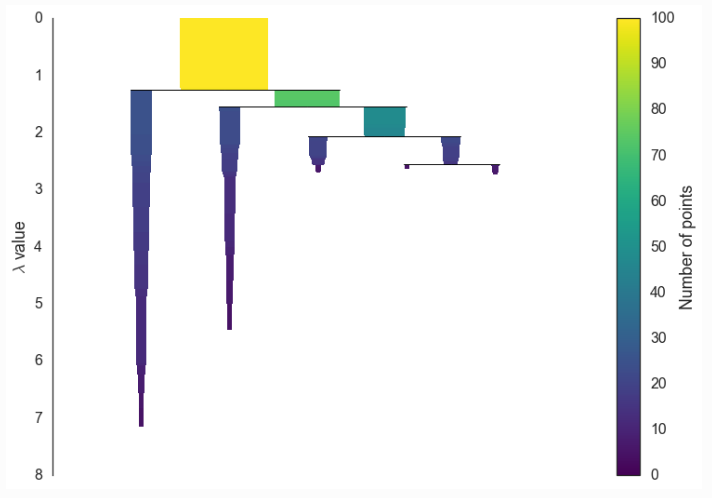
\includegraphics[width=0.5\textwidth]{hdbscan_3}
    \caption{Condensed cluster hierarchy. Source\cite{how_hdbscan_works}}
    \label{fig:hdbscan_3}
\end{figure}

The fourth step consists of condensing the previously built cluster hierarchy into a smaller tree.
The process starts at the top where all vertices still belong to the same cluster.
Iterating through the hierarchy,
for each split the two resulting clusters are compared against a predefined minimum cluster size.
If the size of a cluster is below the minimum,
its points will be discarded, while the other cluster remains in the parent cluster.
If both cluster sizes are above or equal the minimum, the clusters are considered as true clusters.
This is repeated until no more splits can be made.

\subparagraph{5. Extract the clusters}
The extraction of the final clusters from the condensed tree is based on the stability per cluster
and once it is selected, none of its subclusters can be chosen.
The stability is based on the persistence of a cluster,
which is measured by $\lambda = \frac{1}{distance}$. The stability for a cluster $C$ is defined as

\begin{equation}
\sum_{p \in \text{C}}^{|C|} ({\lambda}_{p} - {\lambda}_{birth})
\end{equation}

where ${\lambda}_{p}$ describes when point $p$ fell out of the cluster and $ {\lambda}_{birth}$
describes when the cluster was created.
Now calculating the stability for each cluster starts at the leaf nodes and ends when the root is reached.
A cluster is selected if its stability is larger the sum of stabilities of its children.
If the sum child stabilities is larger than that of its parent,
the parent stability will be set to the value of the sum of its children,
but no selection will be done.
Based on this approach the final clusters will be selected, with regards to varying densities and noise.
